\documentclass[11pt, a4paper]{article}
\usepackage[utf8]{inputenc}
\usepackage{graphicx}
\usepackage{fancyhdr}
\usepackage{amssymb}
\usepackage{amsmath}
\usepackage{amsthm}
\usepackage{mathrsfs}
\usepackage{float}
\usepackage{tikz}
\usetikzlibrary{automata,arrows}
\graphicspath{{./images/}}

\usepackage{gfsartemisia-euler}
\usepackage[T1]{fontenc}
\input{~/tex-defaults/LaTeX-Math-Commands/math/x308-math.sty}
\setMathFootnotes
\input{~/tex-defaults/LaTeX-Math-Commands/math/extended/x308-model_theory.sty}

\usepackage{listings}

%%%%%%%%%%%%%%%%%%%%%%%%%%%%%%%%%%%%%%%%%%%%%%
%%%%%%%%%%          CONFIG          %%%%%%%%%%
\newcommand{\settingsTitle}{Title}
\newcommand{\settingsFirstName}{First}
\newcommand{\settingsLastName}{Last}
\newcommand{\settingsMonth}{Month}
\newcommand{\settingsYear}{Year}
\newcommand{\settingsCourseDept}{Dept}
\newcommand{\settingsCourseNum}{Num} % DON'T FORGET `\_'
\newcommand{\settingsQuarter}{Quarter}
%%%%%%%%%%          CONFIG          %%%%%%%%%%
%%%%%%%%%%%%%%%%%%%%%%%%%%%%%%%%%%%%%%%%%%%%%%

% create title
\title{\settingsTitle}
\author{\settingsFirstName\,\settingsLastName}
\date{\settingsMonth\,\settingsYear}

\begin{document}

% set pagestyle
\pagestyle{fancy}
\setlength{\headheight}{14pt}

% clear header
\fancyhead{}

% set header
\fancyhead[L]{\settingsCourseDept\,\settingsCourseNum\, | \settingsQuarter\,\settingsYear}
\fancyhead[R]{\settingsLastName}

% homework title
\maketitle
% ensure titlepage has same style
\thispagestyle{fancy}

\begin{theorem}
    This is true.
\end{theorem}

\begin{proof}
    The proof is left as an exercise to the reader.
\end{proof}

\begin{table}[H]
    \begin{tabular}{|l|l|l|}
        \hline
        a   & b & c \\ \hline
        d   & e & f \\ \hline
        g   & h & i  \\ \hline
    \end{tabular}
    \caption{Caption.}
    \label{tbl:LABEL}
\end{table}

\begin{figure}[H]
    \centering
    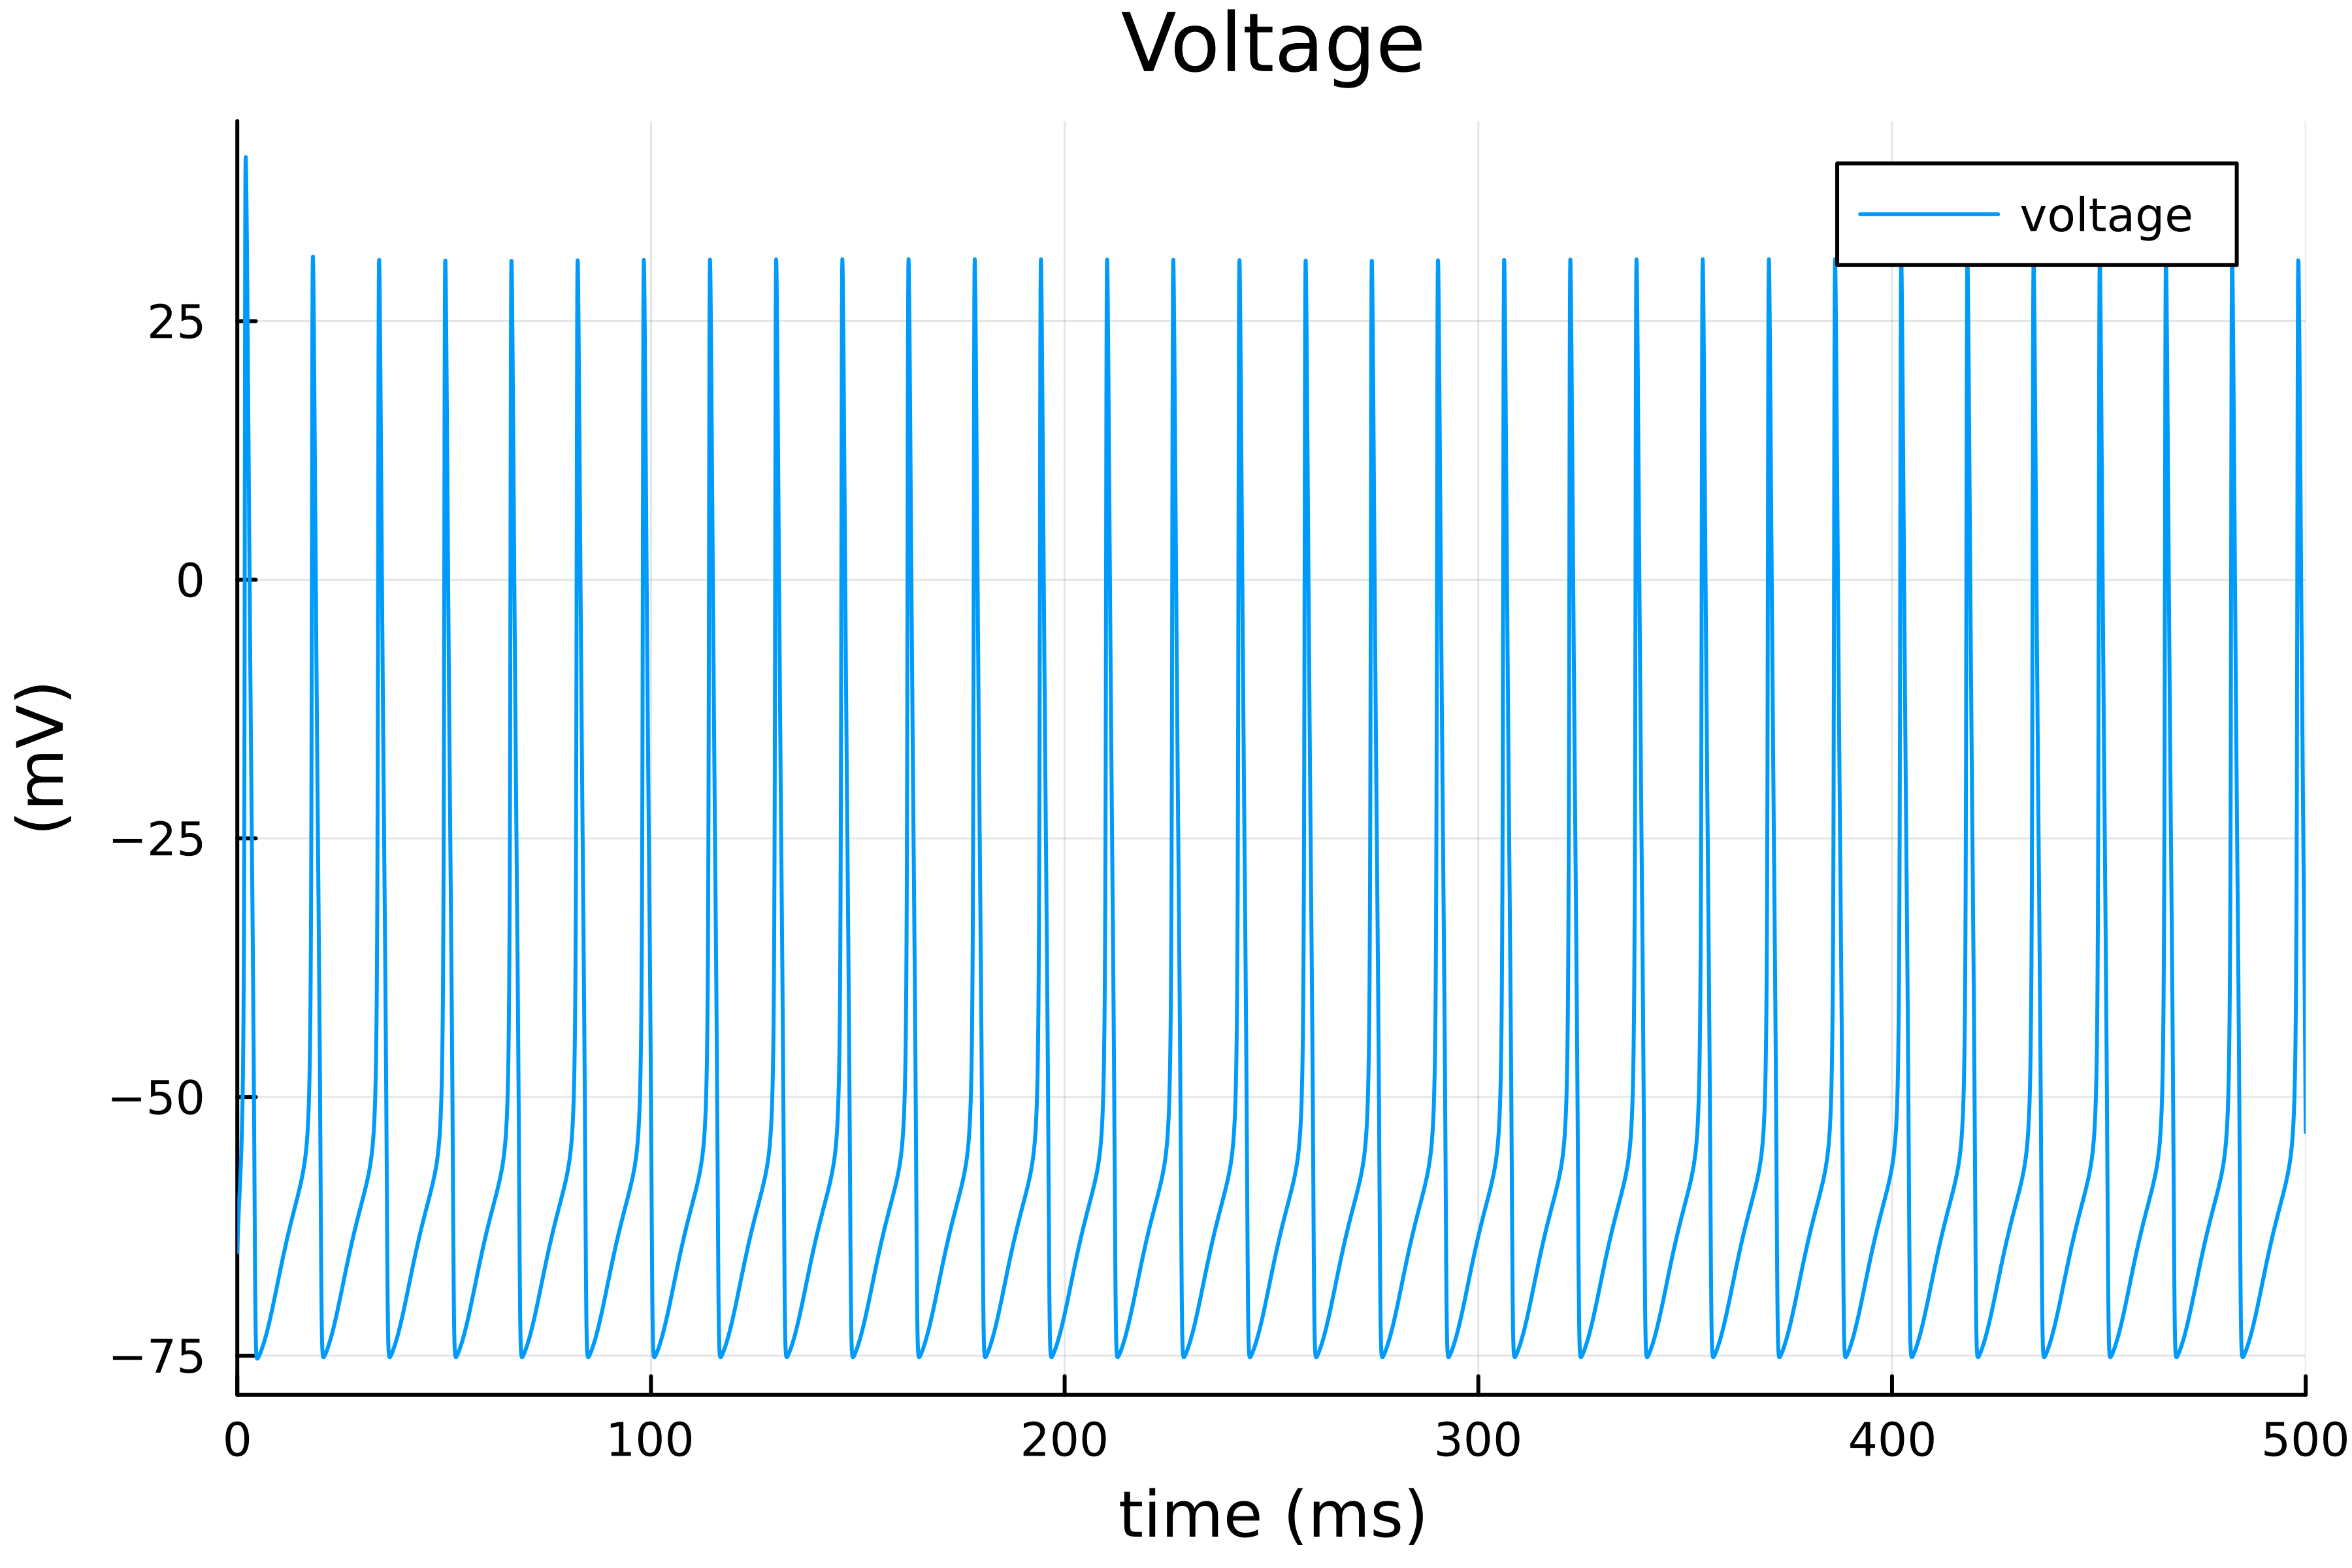
\includegraphics[width=0.75\columnwidth]{example.png}
    \caption{Caption.}
    \label{fig:LABEL}
\end{figure}

\begin{figure}[H]
    \begin{tikzpicture}[>=stealth',shorten >=1pt,auto,node distance=5 cm, scale = 1, transform shape]

        \node[initial,state]    (A)                 {$s_0$};
        \node[state]            (B) [right of=A]    {$s_2$};
        \node[state,accepting]  (C) [above of=B]    {$s_1$};
        \node[state,accepting]  (D) [below of=B]    {$s_3$};
        
        \path[->] (A) edge [left]   node [align=center]  {$ c = c + 1 $} (C)
              (A) edge [above]      node [align=center]  {$ c = c + 5 $} (B)
              (A) edge [left]       node [align=center]  {$ c = c - 1 $} (D)
              (B) edge [right]      node [align=center]  {$ c = c - 1 $} (D)
              (C) edge [loop above] node [align=center]  {$ c = c + 1 $} (C)
              (D) edge [loop below] node [align=center]  {$ c = c - 2 $} (D);
        
        \end{tikzpicture}

    \caption{Caption.}
    \label{fig:LABEL2}
\end{figure}

\end{document}
